\documentclass{article}
\usepackage[utf8]{inputenc}
\usepackage[L7x]{fontenc}
\usepackage[lithuanian]{babel}
\usepackage{lmodern}
\usepackage{color}
\usepackage{tikz}
\usetikzlibrary{positioning}% we need to add block on the right of next block
\usepackage{comment}
\usepackage{animate}
\usepackage{ifthen}
\usepackage{indentfirst}
\usepackage{mdframed}
\usepackage[many]{tcolorbox} 
\usepackage{empheq}
\usepackage{hyperref}
\usetikzlibrary{arrows} %geogebra

\begin{document}
\tcbset{highlight math style={enhanced,
  colframe=red!60!black,colback=yellow!50!white,arc=4pt,boxrule=1pt}} %highlight of equations
  
\newcommand{\go}[2]{
\hyperlink{#2}{
\begin{tikzpicture}
%\draw[right, rounded corners=0.2cm] (#1) rectangle node{\hypertarget{#1}{\tbf{GO}}};
\node[rectangle, draw=black, fill=blue!30, rounded corners=.2cm] (#1) {\hypertarget{#1}{\textbf{GO}}};
\end{tikzpicture}}}

\newcommand{\back}[2]{
\hyperlink{#2}{\begin{tikzpicture}
\node[rectangle, draw=black, fill=red!30, minimum size=2cm] (#1) {\hypertarget{#1}{\textbf{BACK}}};
\end{tikzpicture}}}

\newcommand{\linego}[2]{
\hyperlink{#2}{
\begin{tikzpicture}
\draw[thick,->] (0,0) -- (0,4.5) (#1) {\hypertarget{#1}{\textbf{GO}}};
%\node[rectangle, draw=black, fill=blue!30, rounded corners=.2cm] (#1) {\hypertarget{#1}{\tbf{GO}}};
\end{tikzpicture}}}

\newcommand{\lineback}[2]{
\hyperlink{#2}{\begin{tikzpicture}
\draw[thick,->] (0,0) -- (0,4.5) (#1) {\hypertarget{#1}{\textbf{BACK}}};
%\node[rectangle, draw=black, fill=red!30, minimum size=2cm] (#1) {\hypertarget{#1}{\tbf{BACK}}};
\end{tikzpicture}}}

%\go{ty1}{ty1b}
%\linego{ty1}{ty1b}
%\lineback{ty1b}{ty1}
%(m-2-1) edge node[above] {$R$} (m-1-2)

\section{Funkcijų transformacijos}
\begin{comment}
\hyperlink{atgal}{
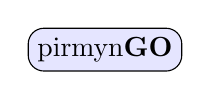
\begin{tikzpicture}
%\draw[right, rounded corners=0.2cm] (#1) rectangle node{\hypertarget{#1}{\tbf{GO}}};
\node[rectangle, draw=black, fill=blue!10, rounded corners=.2cm] (pirmyn) {\hypertarget{pirmyn}{\textbf{GO}}};
\end{tikzpicture}}

\hyperlink{atgal}{
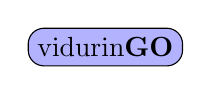
\begin{tikzpicture}
%\draw[right, rounded corners=0.2cm] (#1) rectangle node{\hypertarget{#1}{\tbf{GO}}};
\node[rectangle, draw=black, fill=blue!30, rounded corners=.2cm] (vidurin) {\hypertarget{vidurin}{\textbf{GO}}};
\end{tikzpicture}}

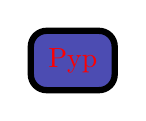
\begin{tikzpicture}
\node[red,draw=black, rounded corners=.2cm, line width=0.8mm, fill=blue!70!yellow] (x) at (5,2) {$\colorbox{blue!70!yellow}{\text{Pyp}}$};
\end{tikzpicture}

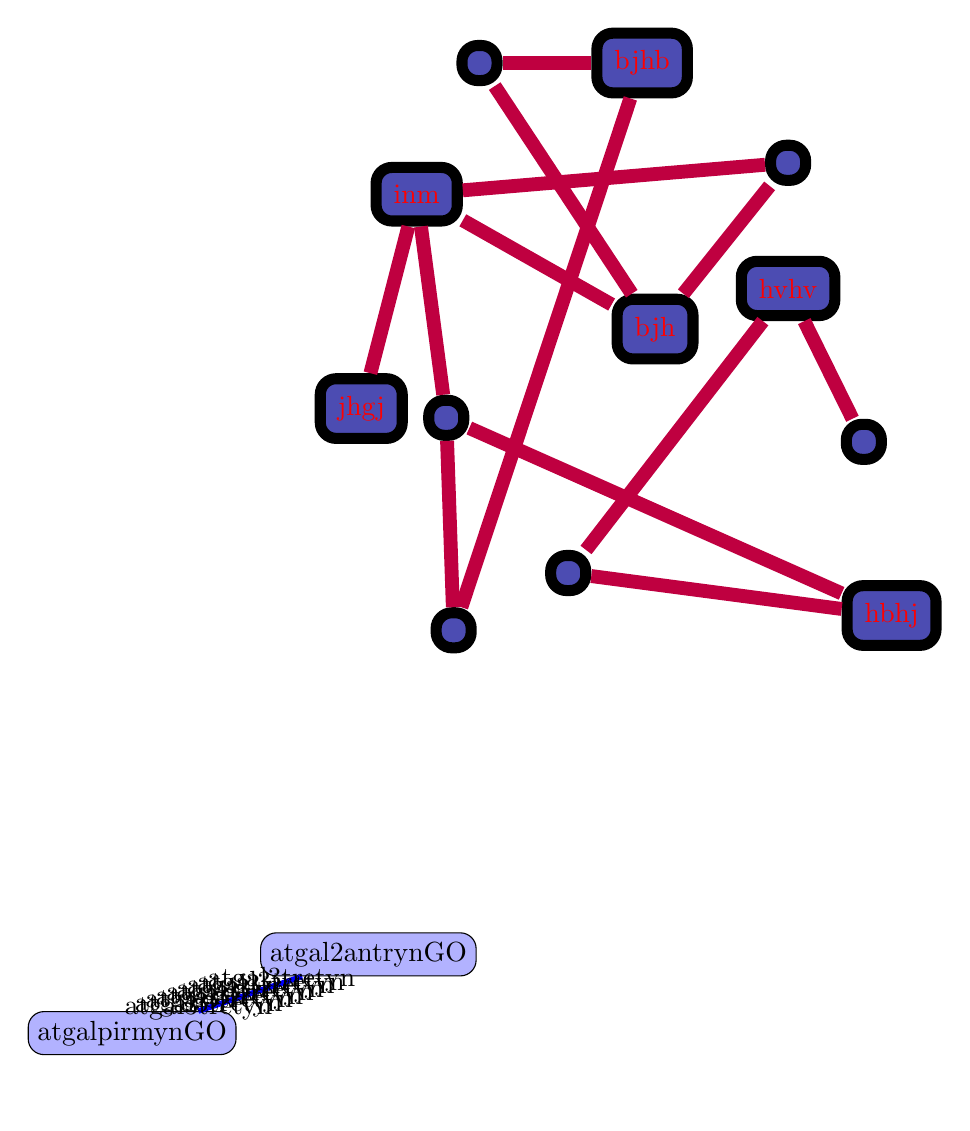
\begin{tikzpicture}
%\draw[right, rounded corners=0.2cm] (#1) rectangle node{\hypertarget{#1}{\tbf{GO}}};
%\hyperlink<1>{atgal}{\node[rectangle, draw=black, fill=blue!30, rounded corners=.2cm]  at (3,0) (vidurin) {\hypertarget{vidurin}{\tbf{GO}}};}
\node[red,draw=black, rounded corners=.2cm, line width=1.408mm, fill=blue!70!yellow] (leaf1) at  (3.613866666666667, 10.653866666666667)  {$\colorbox{blue!70!yellow}{\text{inm}}$};
\node[red,draw=black, rounded corners=.2cm, line width=1.408mm, fill=blue!70!yellow] (leaf2) at  (2.9098666666666673, 7.931733333333334)  {$\colorbox{blue!70!yellow}{\text{jhgj}}$};
\node[red,draw=black, rounded corners=.2cm, line width=1.408mm, fill=blue!70!yellow] (leaf3) at  (9.6448, 5.303466666666667)  {$\colorbox{blue!70!yellow}{\text{hbhj}}$};
\node[red,draw=black, rounded corners=.2cm, line width=1.408mm, fill=blue!70!yellow] (leaf4) at  (6.641066666666667, 8.940800000000001)  {$\colorbox{blue!70!yellow}{\text{bjh}}$};
\node[red,draw=black, rounded corners=.2cm, line width=1.408mm, fill=blue!70!yellow] (leaf5) at  (8.330666666666668, 9.457066666666668)  {$\colorbox{blue!70!yellow}{\text{hvhv}}$};
\node[red,draw=black, rounded corners=.2cm, line width=1.408mm, fill=blue!70!yellow] (leaf6) at  (6.476800000000001, 12.32)  {$\colorbox{blue!70!yellow}{\text{bjhb}}$};
\node[red,draw=black, rounded corners=.2cm, line width=1.408mm, fill=blue!70!yellow] (leaf7) at  (4.411733333333333, 12.32)  {$\colorbox{blue!70!yellow}{\text{}}$};
\node[red,draw=black, rounded corners=.2cm, line width=1.408mm, fill=blue!70!yellow] (leaf8) at  (4.083200000000001, 5.115733333333334)  {$\colorbox{blue!70!yellow}{\text{}}$};
\node[red,draw=black, rounded corners=.2cm, line width=1.408mm, fill=blue!70!yellow] (leaf9) at  (5.538133333333334, 5.8432)  {$\colorbox{blue!70!yellow}{\text{}}$};
\node[red,draw=black, rounded corners=.2cm, line width=1.408mm, fill=blue!70!yellow] (leaf10) at  (9.292800000000002, 7.509333333333334)  {$\colorbox{blue!70!yellow}{\text{}}$};
\node[red,draw=black, rounded corners=.2cm, line width=1.408mm, fill=blue!70!yellow] (leaf11) at  (8.330666666666668, 11.0528)  {$\colorbox{blue!70!yellow}{\text{}}$};
\node[red,draw=black, rounded corners=.2cm, line width=1.408mm, fill=blue!70!yellow] (leaf12) at  (3.989333333333333, 7.8144)  {$\colorbox{blue!70!yellow}{\text{}}$};
\draw[line width=1.76mm, purple, solid] (leaf1) -- (leaf2);
\draw[line width=1.76mm, purple, solid] (leaf8) -- (leaf12);
\draw[line width=1.76mm, purple, solid] (leaf3) -- (leaf9);
\draw[line width=1.76mm, purple, solid] (leaf5) -- (leaf10);
\draw[line width=1.76mm, purple, solid] (leaf4) -- (leaf11);
\draw[line width=1.76mm, purple, solid] (leaf6) -- (leaf7);
\draw[line width=1.76mm, purple, solid] (leaf11) -- (leaf1);
\draw[line width=1.76mm, purple, solid] (leaf3) -- (leaf12);
\draw[line width=1.76mm, purple, solid] (leaf5) -- (leaf9);
\draw[line width=1.76mm, purple, solid] (leaf4) -- (leaf7);
\draw[line width=1.76mm, purple, solid] (leaf6) -- (leaf8);
\draw[line width=1.76mm, purple, solid] (leaf12) -- (leaf1);
\draw[line width=1.76mm, purple, solid] (leaf4) -- (leaf1);
\node[rectangle, draw=black, fill=blue!30, rounded corners=.2cm] at (0,0) (pirmyn) {\hyperlink{atgal}{\hypertarget{pirmyn}{\tbf{GO}}}};
\node[rectangle, draw=black, fill=blue!30, rounded corners=.2cm] at (3,1) (antryn) {\hyperlink{atgal2}{\hypertarget{antryn}{\tbf{GO}}}};
%\path (pirmyn) edge [line width=2pt, draw=blue] node [pos=0, circle] {\hyperlink{atgal3}{\hypertarget{tretyn}{\phantom{X}}}} node [pos=.2, circle] {\hyperlink{atgal3}{\hypertarget{tretyn}{\phantom{X}}}} node [pos=.4, circle]{\hyperlink{atgal3}{\hypertarget{tretyn}{\phantom{X}}}} node [pos=.6, circle] {\hyperlink{atgal3}{\hypertarget{tretyn}{\phantom{X}}}} node [pos=.8, circle] {\hyperlink{atgal3}{\hypertarget{tretyn}{\phantom{X}}}} node [pos=1, circle] {\hyperlink{atgal3}{\hypertarget{tretyn}{\phantom{X}}}}  (antryn);
\draw[line width=2pt, draw=blue]  (pirmyn) -- (antryn) 
\foreach \i in {1,...,9} { node [pos=\i/10, circle] {\hyperlink{atgal3}{\hypertarget{tretyn}{\phantom{X}}} }};
\end{tikzpicture}

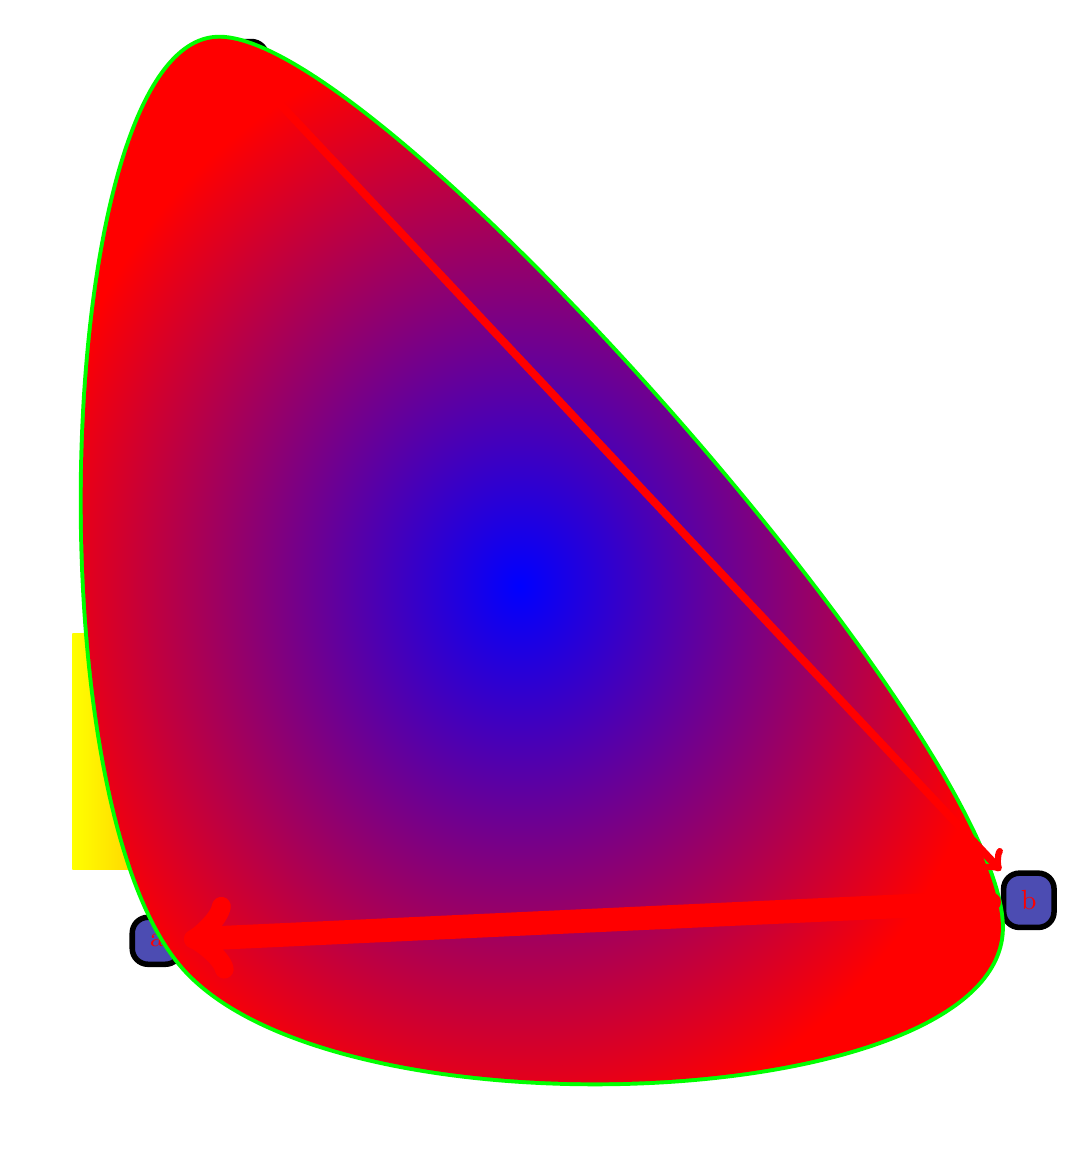
\begin{tikzpicture}
%\fill [black] (-1,-1) rectangle (1,1);
%\shade [color=white] (-1,-1) rectangle (1,1);
%\shade [ball color=white] (-1,-1) rectangle (1,1);
%\shade [ball color=white] (0,0) circle [radius=1cm];
%\shade[top color=blue,bottom color=red] (0,0) rectangle (4,4);
\shade[left color=yellow,right color=red] (-1,1) rectangle (4,4);
\node[red,draw=black, rounded corners=.2cm, line width=0.702mm, fill=blue!70!yellow] (x) at  (0.0702, 0.0936)  {$\colorbox{blue!70!yellow}{\text{a}}$};
\node[red,draw=black, rounded corners=.2cm, line width=0.702mm, fill=blue!70!yellow] (y) at  (11.1466, 0.608)  {$\colorbox{blue!70!yellow}{\text{b}}$};
\node[red,draw=black, rounded corners=.2cm, line width=0.702mm, fill=blue!70!yellow] (z) at  (1.17, 11.216)  {$\colorbox{blue!70!yellow}{\text{c}}$};
\draw [line width=1mm, green, fill=yellow] plot [smooth cycle, tension=0.7] coordinates {(x.south east) (y.south west) (z.north west)};
\shade[inner color=blue,outer color=red] plot [smooth cycle, tension=0.7] coordinates {(x.south east) (y.south west) (z.north west)};
\draw[line width=1mm, red, solid,<->,line width=3mm] (x) -- (y);
\draw[line width=1mm, red, solid,<->] (y) -- (z);
\end{tikzpicture}
\end{comment}
\subsection{4 pagrindinės funkcijų transformacijos}
\begin{itemize}
\item \fbox{$x \rightarrow x+c$} paslinkimas $c$ vienetų kairėn. \go{t1}{t1b}
\item \fbox{$f(x) \rightarrow f(x)+c$} paslinkimas $c$ vienetų viršun. \go{t2}{t2b}
\item \fbox{$x \rightarrow kx$} artinimas $k$ kartų prie $y$ ašies. \go{t3}{t3b}
\item \fbox{$f(x) \rightarrow kf(x)$} tolinimas $k$ kartų nuo $x$ ašies. \go{t4}{t4b}
\end{itemize}

\subsection{Papildomos funkcijų transformacijos}
\begin{itemize}
\item \fbox{$f(x) \rightarrow |f(x)|$} atspindys nuo $x$ ašies į teigiamą sritį.
\item \fbox{$f(x) \rightarrow f^{-1}(x)$} simetrija tiesės $y=x$ atžvilgiu
\end{itemize}

\subsection{Integralai}

Integralu $\displaystyle \int_a^b f(x)dx$ laikomas srities tarp $Ox$ ašies ir $f(x)$ plotas, kai $x \in [a,b]$ \go{i1}{i1b}

\begin{comment}
\newpage
\hyperlink{pirmyn}{
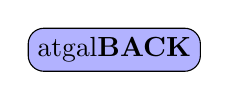
\begin{tikzpicture}
%\draw[right, rounded corners=0.2cm] (#1) rectangle node{\hypertarget{#1}{\tbf{GO}}};
\node[rectangle, draw=black, fill=blue!30, rounded corners=.2cm] (atgal) {\hypertarget{atgal}{\textbf{BACK}}};
\end{tikzpicture}}

\newpage
\hyperlink{antryn}{
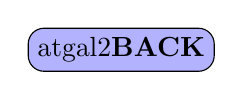
\begin{tikzpicture}
%\draw[right, rounded corners=0.2cm] (#1) rectangle node{\hypertarget{#1}{\tbf{GO}}};
\node[rectangle, draw=black, fill=blue!30, rounded corners=.2cm] (atgal2) {\hypertarget{atgal2}{\textbf{BACK}}};
\end{tikzpicture}}
\end{comment}

\newpage
\hyperlink{tretyn}{
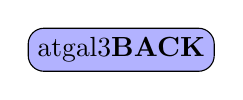
\begin{tikzpicture}
%\draw[right, rounded corners=0.2cm] (#1) rectangle node{\hypertarget{#1}{\tbf{GO}}};
\node[rectangle, draw=black, fill=blue!30, rounded corners=.2cm] (atgal3) {\hypertarget{atgal3}{\textbf{BACK}}};
\end{tikzpicture}}
\pgfkeys{/pgf/number format/.cd,fixed relative,precision=3}

\subsection{Paslinkimas $c$ vienetų kairėn}
  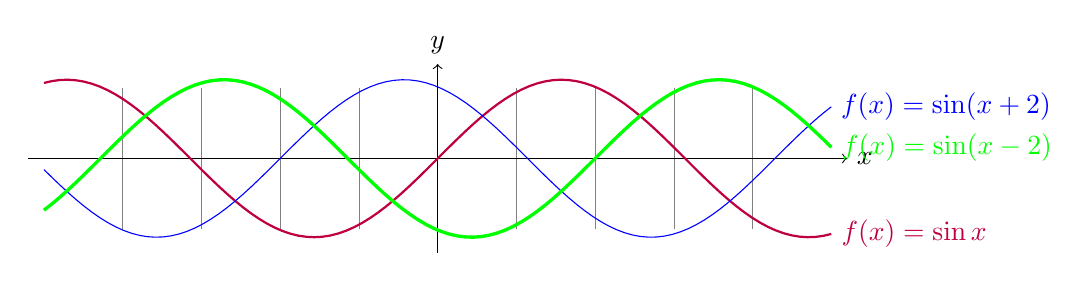
\begin{tikzpicture}[domain=-5:5,samples=100] 
    \draw[very thin,color=gray] (-4.9,-0.9) grid (4.9,0.9);
    \draw[->] (-5.2,0) -- (5.2,0) node[right] {$x$}; 
    \draw[->] (0,-1.2) -- (0,1.2) node[above] {$y$};
    \draw[thick, color=purple]   plot (\x,{sin(\x r)})    node[right] {$f(x) = \sin x$}; 
    \draw[color=blue]   plot (\x,{sin(deg(\x+2))})    node[right] {$f(x) = \sin (x+2)$}; 
    \draw[very thick, color=green]   plot (\x,{sin(deg(\x-2))})    node[right] {$f(x) = \sin (x-2)$}; 
  \end{tikzpicture}

\newcounter{k}
\setcounter{k}{-15}

\back{t1b}{t1}

\begin{animateinline}[controls,autoplay,palindrome]{10}%
  \whiledo{\thek<17}{%
  \begin{tikzpicture}[domain=-5:5,samples=100]%
    \draw[very thin,color=gray] (-4.9,-0.9) grid (4.9,0.9);%
    \draw[->] (-5.2,0) -- (5.2,0) node[right] {$x$};%
    \draw[->] (0,-1.5) -- (0,1.5) node[above] {$y$};%
    \pgfmathsetmacro\result{\thek/10};%
    \ifthenelse{\thek<0}{%
    \draw[thick, color=purple]   plot (\x,{sin(deg(\x+\thek/10)})    node[right, minimum height=0.7cm, minimum width=4cm] {$f(x) = \sin (x\pgfmathprintnumber{\result})$};}%
   {\draw[thick, color=purple]   plot (\x,{sin(deg(\x+\thek/10)})    node[right, minimum height=0.7cm, minimum width=4cm] {$f(x) = \sin (x+\pgfmathprintnumber{\result})$};}%
  \end{tikzpicture}%
  \stepcounter{k}%
  \ifthenelse{\thek<17}{\newframe}{\end{animateinline}}}%

\newpage
\subsection{Paslinkimas $c$ vienetų viršun}

  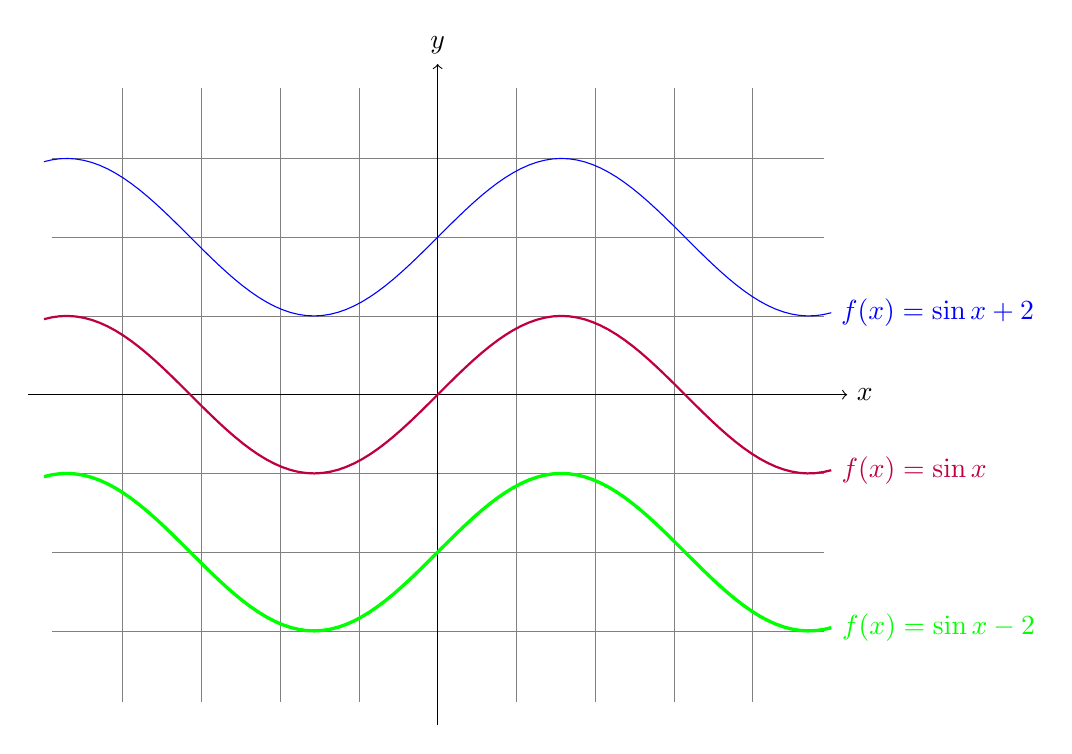
\begin{tikzpicture}[domain=-5:5,samples=100] 
    \draw[very thin,color=gray] (-4.9,-3.9) grid (4.9,3.9);
    \draw[->] (-5.2,0) -- (5.2,0) node[right] {$x$}; 
    \draw[->] (0,-4.2) -- (0,4.2) node[above] {$y$};
    \draw[thick, color=purple]   plot (\x,{sin(\x r)})    node[right] {$f(x) = \sin x$}; 
    \draw[color=blue]   plot (\x,{sin(deg(\x))+2})    node[right] {$f(x) = \sin x +2$}; 
    \draw[very thick, color=green]   plot (\x,{sin(deg(\x))-2})    node[right] {$f(x) = \sin x-2$}; 
  \end{tikzpicture}
  
\setcounter{k}{-15}
\back{t2b}{t2}

\begin{animateinline}[controls,autoplay,palindrome]{10}
  \whiledo{\thek<17}{%
  \begin{tikzpicture}[domain=-5:5,samples=100]%
    \draw[very thin,color=gray] (-4.9,-2.9) grid (4.9,2.9);%
    \draw[->] (-5.2,0) -- (5.2,0) node[right] {$x$};%
    \draw[->] (0,-2.9) -- (0,2.9) node[above] {$y$};%
    \pgfmathsetmacro\result{\thek/10};%
    \ifthenelse{\thek<0}{%
    \draw[thick, color=purple]   plot (\x,{sin(deg(\x))+\thek/10})    node[right, minimum height=0.7cm, minimum width=4cm] {$f(x) = \sin (x)\pgfmathprintnumber{\result}$};}%
   {\draw[thick, color=purple]   plot (\x,{sin(deg(\x))+\thek/10})    node[right, minimum height=0.7cm, minimum width=4cm] {$f(x) = \sin (x)+\pgfmathprintnumber{\result}$};}%
  \end{tikzpicture}%
  \stepcounter{k}%
  \ifthenelse{\thek<17}{\newframe}{\end{animateinline}}}%


\newpage
\subsection{Artinimas $k$ kartų prie $y$ ašies}
  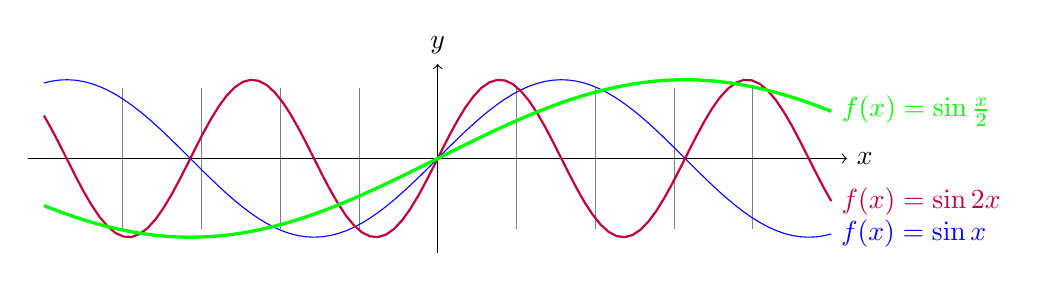
\begin{tikzpicture}[domain=-5:5,samples=100] 
    \draw[very thin,color=gray] (-4.9,-0.9) grid (4.9,0.9);
    \draw[->] (-5.2,0) -- (5.2,0) node[right] {$x$}; 
    \draw[->] (0,-1.2) -- (0,1.2) node[above] {$y$};
    \draw[color=blue]   plot (\x,{sin(\x r)})    node[right] {$f(x) = \sin x$}; 
    \draw[thick, color=purple]   plot (\x,{sin(2*\x r)})    node[right] {$f(x) = \sin 2x$}; 
    \draw[very thick, color=green]   plot (\x,{sin(\x/2 r)})    node[right] {$f(x) = \sin \frac{x}{2}$}; 
  \end{tikzpicture}
\setcounter{k}{-40}

\back{t3b}{t3}

\begin{animateinline}[controls,autoplay,palindrome]{20}%
  \whiledo{\thek<40}{%
  \begin{tikzpicture}[domain=-30:30,samples=200] %
    %\useasboundingbox (-0.5\textwidth,-2) rectangle (\textwidth,3.28);
    \pgfmathsetmacro\result{\thek/10};%
    \begin{scope}[scale=0.15, local bounding box=scope1]
    \draw[very thin,color=gray,ystep=10] (-29.9,-4.9) grid (29.9,4.9);%
    \draw[->] (-29.2,0) -- (29.2,0) node[right] {$x$};%
    \draw[->] (0,-4.9) -- (0,4.9) node[above] {$y$};%
    \draw[thick, color=purple]   plot (\x,{5*sin(deg(\x*\thek/10))});
    \end{scope}
    \node[right = 0cm of scope1, color=purple, minimum height=0.7cm, minimum width=3.5cm] {$f(x) = \sin (\pgfmathprintnumber{\result} x)$};%
  \end{tikzpicture}%
  \stepcounter{k}%
  \ifthenelse{\thek<40}{\newframe}{\end{animateinline}}}%


\newpage
\subsection{Tolinimas $k$ kartų nuo $x$ ašies}
  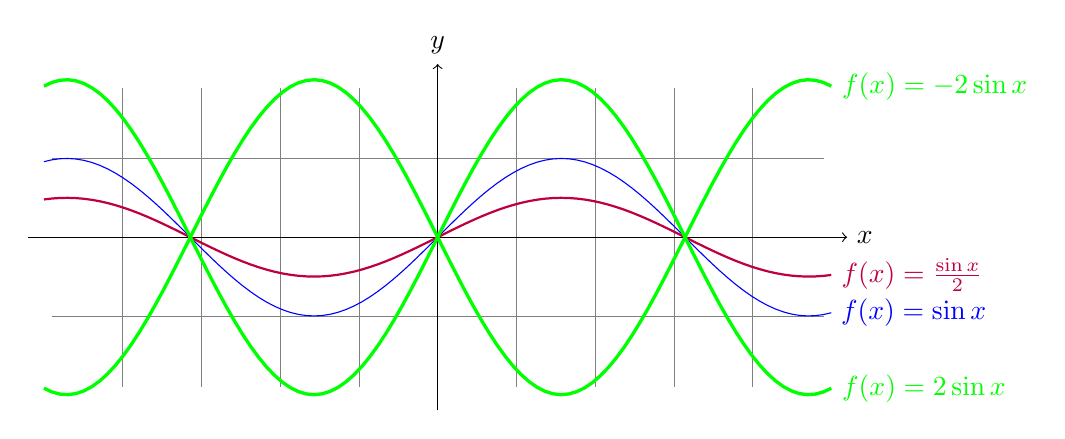
\begin{tikzpicture}[domain=-5:5,samples=100] 
    \draw[very thin,color=gray] (-4.9,-1.9) grid (4.9,1.9);
    \draw[->] (-5.2,0) -- (5.2,0) node[right] {$x$}; 
    \draw[->] (0,-2.2) -- (0,2.2) node[above] {$y$};
    \draw[color=blue]   plot (\x,{sin(\x r)})    node[right] {$f(x) = \sin x$}; 
    \draw[thick, color=purple]   plot (\x,{sin(\x r)/2})    node[right] {$f(x) = \frac{\sin x}{2}$}; 
    \draw[very thick, color=green]   plot (\x,{sin(\x r)*2})    node[right] {$f(x) = 2\sin x$}; 
    \draw[very thick, color=green]   plot (\x,{sin(\x r)*(-2)})    node[right] {$f(x) = -2\sin x$}; 
  \end{tikzpicture}

\back{t4b}{t4}

\setcounter{k}{-15}
\begin{animateinline}[controls,autoplay,palindrome]{10}%
  \whiledo{\thek<17}{
  \begin{tikzpicture}[domain=-5:5,samples=100] 
    \draw[very thin,color=gray] (-4.9,-1.9) grid (4.9,1.9);%
    \draw[->] (-4.2,0) -- (5.2,0) node[right] {$x$};% 
    \draw[->] (0,-2.2) -- (0,2.2) node[above] {$y$};%
    \pgfmathsetmacro\result{\thek/10};%
    \draw[thick, color=purple]   plot (\x,{\thek/10*sin(deg(\x))})    node[right, color=purple, minimum height=0.7cm, minimum width=3.5cm] {$f(x) = \pgfmathprintnumber\result\cdot\sin x$};%
  \end{tikzpicture}%
  \stepcounter{k}%
  \ifthenelse{\thek<17}{\newframe}{\end{animateinline}}}

\end{document}